\documentclass[11pt]{beamer}
%\usefonttheme{professionalfonts}
\usefonttheme{serif}

\usepackage[utf8]{inputenc}
\usepackage[T1]{fontenc}
\usepackage{lmodern}
\usepackage[spanish]{babel}
\usepackage{amsmath}
\usepackage{amssymb}
\usetheme{EastLansing}
\usepackage{graphicx}
\usepackage[]{xcolor}
\usepackage{tikz}
\usetikzlibrary{shapes.geometric, arrows}

\author{Dr. Alejandro Rodriguez}
\title{Probabilidad y Estad\'istica\\Probabilidad}
\subtitle{Universidad Tecnol\'ogica Iz\'ucar de Matamoros\\UTIM }


\begin{document}

    \begin{frame}[plain]
        \maketitle
    \end{frame}

    \begin{frame}{Temas de Probabilidad}
      \begin{itemize}
          \item Conjuntos
          \item Probabilidad Básica y Condicional
          \item Distribuciones Discretas de Probabilidad
          \item Distribuciones Continuas de Probabilidad
          \item Distribuciones Muestrales
      \end{itemize}
    \end{frame}
    \begin{frame}{Probabilidad}
       \begin{block}{Probabilidad}
           El término \textbf{probabilidad} se refiere al estudio de azar y la incertidumbre en cualquier
           situación en la cual varios posibles sucesos pueden ocurrir.
       \end{block}
       \pause
       En palabras simples, fenómenos aleatorios son los que pueden dar lugar a varios resultados, sin que pueda ser posible enunciar con certeza cuál de éstos va a ser observado en la realización del experimento.
    \end{frame}



    \section*{Conjuntos}
      \begin{frame}{Espacio muestral}
          \begin{block}{title}
              Definir los conceptos y notación de conjuntos:
              -Universo
              -Vacío
              -Subconjunto

              Describir el proceso de construcción del diagrama de Venn Euler.

              Explicar las operaciones entre conjuntos:
              - Unión
              - Intersección
              - Complemento
              - Diferencia
          \end{block}
      \end{frame}
      \subsection*{Espacio Muestral}
      \begin{frame}{Conjuntos o espacio muestral}
          \begin{block}{Espacio muestral}
              El \textbf{espacio muestral} de un experimento denotado por $E$ , es el \textbf{conjunto} de todos los posibles resultados de dicho experimento.
          \end{block}
          \pause
          Ejemplos:
          \begin{enumerate}[<+->]
              \item El espacio muestral asociado a lanzar un dado, E = {1,2,3,4,5,6}
              \item El espacio asociado a preguntar a un cliente si le gusta o no nuestro producto es E ={S, N} (S – sí; N – no)
              \item El espacio asociado a indagar si 3 clientes que entraron a una tienda compraron un producto es E = {SSS, SSN, SNS, NSS, SNN, NSN, NNS, NNN}.
          \end{enumerate}
      \end{frame}
      \subsection*{Suceso o evento}
      \begin{frame}{Conjuntos: Suceso o evento}
          \begin{block}{Suceso o evento}
              Un \textbf{suceso} o \textbf{evento} es cualquier recopilación (\textbf{subconjunto}) de resultados contenidos en el espacio muestral $E$. Un evento es \textit{simple} si consiste en exactamente un resultado y \textit{compuesto} si consiste en más de un resultado.
          \end{block}
          \pause
          Dado que los sucesos son subconjuntos del espacio muestral, son muy útiles los diagramas de Venn para su representación:
          \begin{figure}
              \centering
              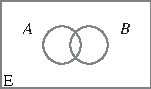
\includegraphics[width=0.3\linewidth]{images/estadistica1}
              \caption{Ejemplo de un diagrama de diagramas de Venn. E. Espacio muestral, A y B representan conjuntos o subconjuntos. }
              \label{fig:estadistica1}
          \end{figure}
      \end{frame}
      \subsection*{Propiedades de conjunto}
      \begin{frame}{}
          \begin{block}{Propiedades de conjunto}
              \begin{enumerate}[<+->]
                  \item El complemento de un evento A, denotado por A', es el conjunto de todos los resultados en \textbf{E} que no están contenidos en A.
                  \item La unión de dos eventos A y B, denotados por A $\cup$ B y leídos “A o B”, es el evento que consiste en todos los resultados que están en A o en B o en ambos eventos
(de tal suerte que la unión incluya resultados donde tanto A como B ocurren, así
también resultados donde ocurre exactamente uno), es decir, todos los resultados
en por lo menos uno de los eventos.
                  \item La intersección de dos eventos A y B, denotada por A $\cap$ B y leída “A y B”, es el
evento que consiste en todos los resultados que están tanto en A como en B.
              \end{enumerate}
          \end{block}
      \end{frame}

      \begin{frame}{Unión}
          \begin{figure}
              \centering
              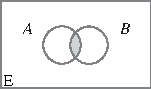
\includegraphics[width=0.7\linewidth]{images/estadistica2}
              \caption{Unión: La región sombreada es A $\cup$ B.}
              \label{fig:estadistica2}
          \end{figure}

      \end{frame}
      \begin{frame}{Intersección}
        \begin{figure}
            \centering
            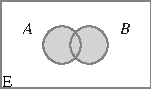
\includegraphics[width=0.7\linewidth]{images/estadistica3}
            \caption{Intersección: La región sombreada es A $\cap$ B}
            \label{fig:estadistica3}
        \end{figure}

      \end{frame}
      \begin{frame}{Complemento}
        \begin{figure}
            \centering
            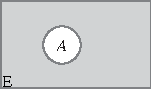
\includegraphics[width=0.7\linewidth]{images/estadistica4}
            \caption{Complemento: La región sombreada es A'. }
            \label{fig:estadistica4}
        \end{figure}

      \end{frame}
      \begin{frame}{Mutuamente excluyentes}
        \begin{figure}
            \centering
            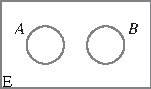
\includegraphics[width=0.7\linewidth]{images/estadistica5}
            \caption{Eventos mutuamente
excluyentes.}
            \label{fig:estadistica5}
        \end{figure}

      \end{frame}

      \begin{frame}{Mutuamente excluyentes}
\textbf{\begin{center}
                 \huge TO BE CONTINUE
\end{center}}
      \end{frame}














    \section*{Probabilidad Básica y Condicional}
      \begin{frame}{title}
        \begin{block}{title}
            content...
        \end{block}
      \end{frame}

    \section*{Distribuciones Discretas de Probabilidad}
    \begin{frame}{title}
        content...
    \end{frame}



    \section*{Distribuciones Continuas de Probabilidad}
    \begin{frame}{title}
        \begin{block}{title}
            content...
        \end{block}
    \end{frame}



    \section*{Distribuciones Muestrales}
    \begin{frame}{title}
        \begin{block}{title}
            content...
        \end{block}
    \end{frame}


\end{document}